\documentclass{exam}

\usepackage{fullpage}
\usepackage{enumerate}
\usepackage{siunitx} 
\usepackage{graphicx}
% \usepackage[fleqn]{amsmath}
\usepackage[fleqn]{mathtools}
\usepackage{cancel}
\usepackage{polynom}
\usepackage{float}
\usepackage{mdwlist}
\usepackage{booktabs}
\usepackage{cancel}
\usepackage{polynom}
\usepackage{caption}

\newcommand{\degree}{\ensuremath{^\circ}} 
\everymath{\displaystyle}

% \begin{figure}[H]
%   \centering
%   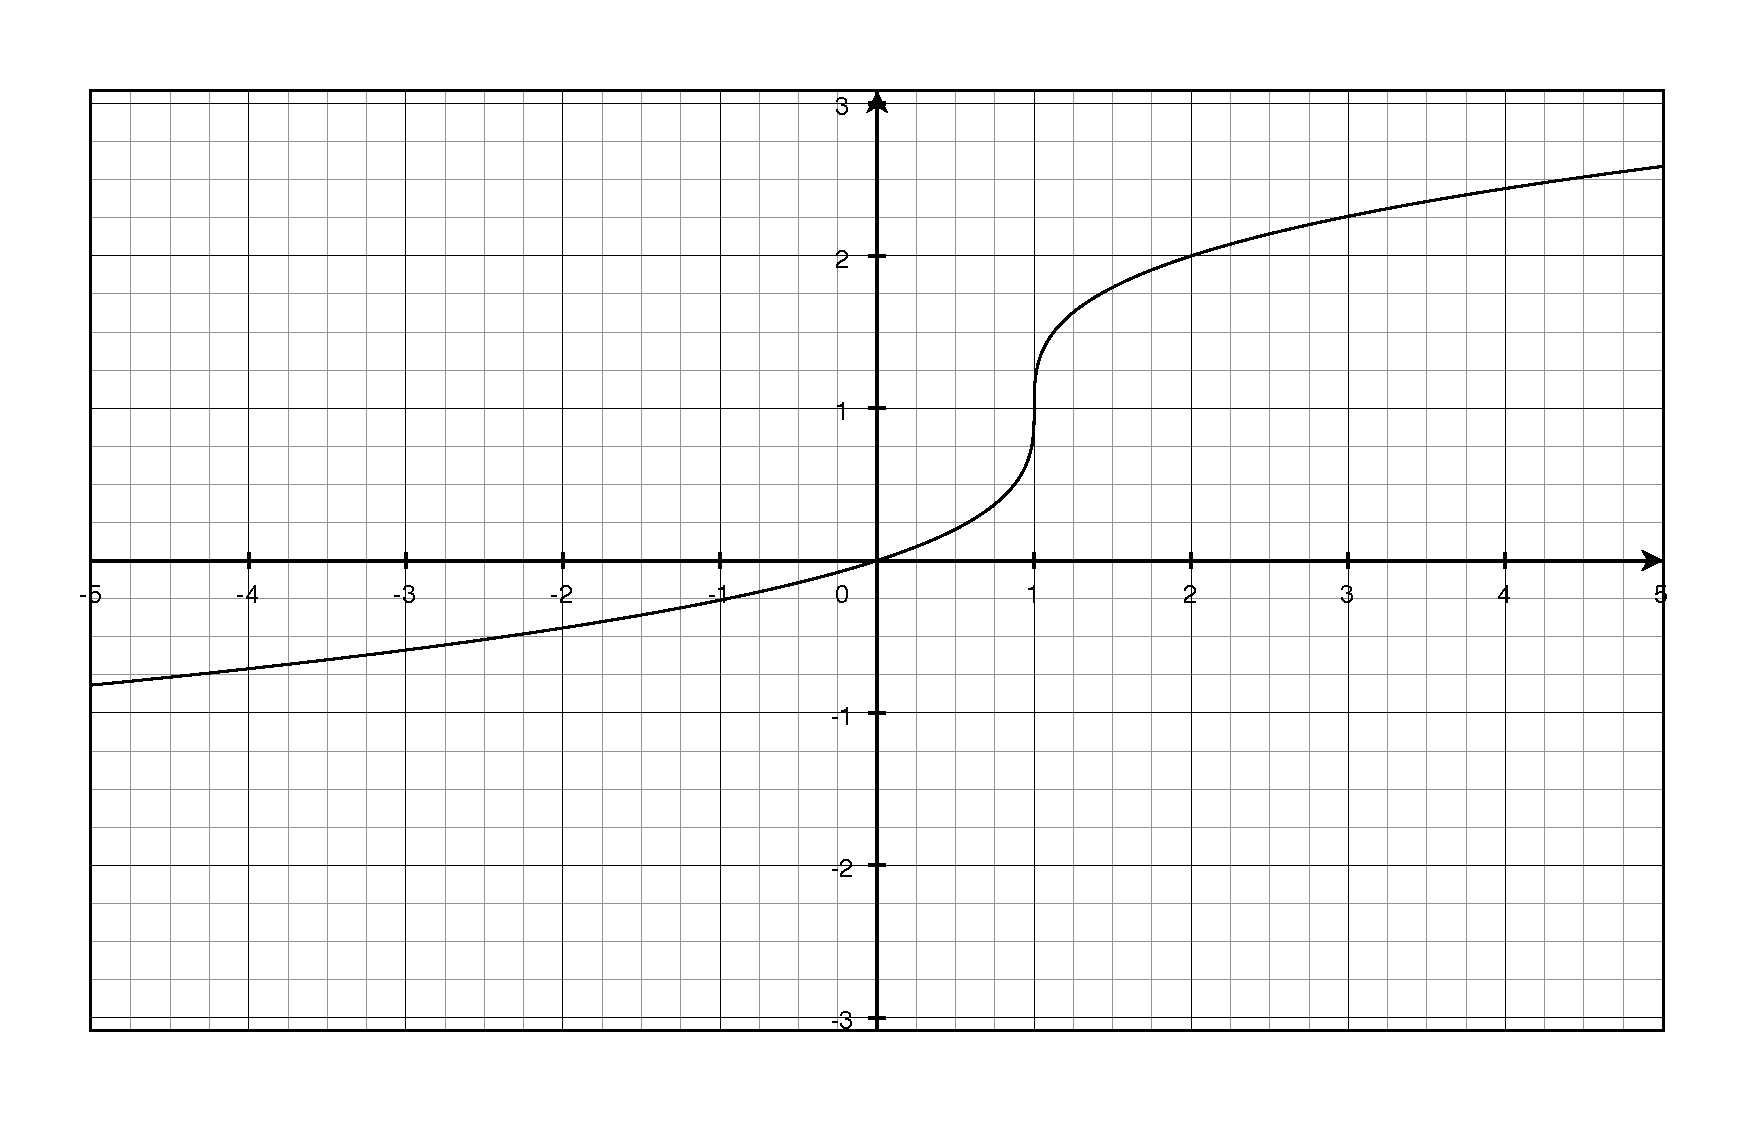
\includegraphics[scale=.3]{question7.eps}
%   \caption*{Question 7}
% \end{figure}

% \begin{tabular}{cc}
% \toprule
% period & amplitude \\
% \midrule
%   $\pi$ & $2$ \\
% \bottomrule
% \end{tabular}

\printanswers

\ifprintanswers 
\usepackage{2in1, lscape} 
\fi

\title{Math 263a \\ Homework 9}
\date{March 21, 2012 \\ Spring Equinox}

\begin{document}

\maketitle

\section{Homework}

\begin{itemize*}
  \item Read Section 3.8
  \item pp. 152-154: 1-12, 15-16, 21-25, 29-30, 33-34, 46
\end{itemize*}

\section{Extra Credit}
Page 153, problem 49
\begin{solution}

If we had an equation for the line which connects the light bulb to the point on the ground, we'd also have a way to
calculate $h$.

The desired line is a tangent line to the circle.  The first thing to do is to find the slope of this line, which we
can do by taking the derivative:
\begin{align*}
  x^2 + y^2 &= 1 \\ 
  \frac{d}{dx} (x^2 + y^2) &= \frac{d}{dx}(1) \\ 
  2x + 2y \frac{dy}{dx} &= 0 \\ 
  \frac{dy}{dx} &= - \frac{x}{y} \\ 
\end{align*}
Let's call $(x_0, y_0)$ the point where the tangent line intersects the circle.  We know the line has to go through both
$(x_0, y_0)$ and $(1.25, 0)$.  We know the slope at this point from the derivative, so the equation for the line is:
\begin{align*}
  y_0 - 0 &= - \frac{x_0}{y_0}(x_0 - 1.25) \\
  y_0^2 &= -x_0^2 + 1.25x_0 \\
\end{align*}
This point is also on the circle, so: $x_0^2 + y_0^2 = 1$.  We now have two equations and two unknowns, so we can find
$x_0$ and $y_0$:
\begin{align*}
  x_0^2 + -x_0^2 + 1.25x_0 &= 1 \\
  x_0 &= \frac{4}{5} \\  
\end{align*}
You can plug $x_0$ back into one of the other equations and find that $y_0 = \frac{3}{5}$.  This means the slope of the
line is:
\[
  m = -\frac{x_0}{y_0} = - \frac{4}{5} \cdot \frac{5}{3} = - \frac{4}{3}
\]
And the equation of the line is:
\begin{align*}
  y &= - \frac{4}{3} \left( x - \frac{5}{4} \right) \\
  y &= -\frac{4}{3} x + \frac{5}{3} \\
\end{align*}
If we plug $x = -2$ into this equation, we get the required height:
\[
  y = -\frac{4}{3} (-2) + \frac{5}{3} = \frac{13}{3}
\]

\end{solution}

\ifprintanswers

\section{Section 3.8}

\begin{description}
\item[1]
\begin{align*}
  y^2 - x^2 &= 1 \\
  2yy' - 2x &= 0 \\
  y' = \frac{x}{y} \\
\end{align*}

\item[2]
\begin{align*}
  9x^2 + 4y^2 &= 36 \\
  18x + 8yy' &= 0 \\
  y' = - \frac{9x}{4y} \\
\end{align*}

\item[3]
\begin{align*}
  xy &= 1 \\
  xy' + y &= 0 \\
  y' = - \frac{y}{x} \\
\end{align*}

\item[4]
\begin{align*}
  x^2 + \alpha^2 y^2 &= 4 \alpha^2 \\
  2x + 2 \alpha^2 yy' &= 0 \\
  y' = - \frac{x}{\alpha^2 y} \\
\end{align*}

\item[5]
\begin{align*}
  xy^2 &= x - 8 \\
  2xyy' + y^2 &= 1 \\
  y' = \frac{1 - y^2}{2xy} \\
\end{align*}

\item[6]
\begin{align*}
  x^2 + 2x^2y + 3xy &= 0 \\
  2x + 2x^2y' + 4xy + 3xy' + 3y &= 0 \\
  y' = \frac{-2x - 4xy - 3y}{2x^2 + 3x} \\
\end{align*}

\item[7]
\begin{align*}
  4x^3 + 7xy^2 &= 2y^3 \\
  12x^2 + 14xyy' + 7y^2 &= 6y^2y' \\
  y' = \frac{12x^2 + 7y^2}{6y^2 - 14xy} \\
\end{align*}

\item[8]
\begin{align*}
  x^2y &= 1 + y^2x \\
  x^2y' + 2xy &= y^2 + 2xyy' \\
  y' &= \frac{y^2 - 2xy}{x^2 - 2xy} \\
\end{align*}

\item[9]
\begin{align*}
  (5xy)^{1/2} + 2y &= y^2 + xy^3 \\
  \frac{1}{2} (5xy)^{-1/2} [5(xy' + y)] + 2y' &= 2yy' + 3xy^2y' + y^3 \\
  % \frac{5(xy' + y)}{2 \sqrt{5xy}} + 2y' - 2yy' - 3xy^2y' &=  y^3 \\
  % \frac{5xy'}{2\sqrt{5xy}} + \frac{5y}{2\sqrt{5xy}} + 2y' - 2yy' - 3xy^2y' &=  y^3 \\
  \frac{5xy'}{2\sqrt{5xy}} + 2y' - 2yy' - 3xy^2y' &=  y^3 - \frac{5y}{2\sqrt{5xy}} \\
  y' = \frac{y^3 - \cfrac{5y}{2\sqrt{5xy}}}{\cfrac{5x}{2\sqrt{5xy}} + 2 - 2y - 3xy^2} \\
\end{align*}

\item[10]
\begin{align*}
  x(y+1)^{1/2} &= xy + 1 \\
  \frac{1}{2}x(y+1)^{-1/2} y' + (y+1)^{1/2} &= xy' + y \\
  \frac{xy'}{2 \sqrt{y+1}} + \sqrt{y+1} &= xy' + y \\
  \frac{xy'}{2 \sqrt{y+1}} - xy' &= y - \sqrt{y+1} \\
  % y' \left( \frac{x}{2 \sqrt{y+1}} - x \right) &= y - \sqrt{y+1} \\
  y' &= \frac{y - \sqrt{y+1}}{\left( \cfrac{x}{2 \sqrt{y+1}} - x \right)} \\
\end{align*}

\item[11]
\begin{align*}
  xy  + \sin(xy) &= 1 \\
  xy' + y + \cos(xy)(xy' + y) &= 0 \\
  xy' + y + xy'\cos(xy) + y \cos(xy) &= 0 \\
  xy' + xy'\cos(xy) &= -y - y \cos(xy) \\
  y'  &= \frac{-y(1 + \cos(xy))}{x(1' + \cos(xy))} \\
  y'  &= - \frac{y}{x} \\
\end{align*}


\item[12]
\begin{align*}
  \cos(xy^2) &= y^2 + x \\
  -\sin(xy^2)(2xyy' + y^2) &= 2yy' + 1 \\
  y' &= - \frac{1 + y^2 \sin(xy^2)}{2y + 2xy \sin(xy^2)}
\end{align*}

\item[15]
\begin{align*}
  \sin(xy) &= y \\
  \cos(xy)(xy' + y) &= y' \\
  y' &= \frac{-y \cos(xy)}{x \cos(xy) - 1} \\
  \\
  y' |_{\left(\frac{\pi}{2}, 1 \right)} &= \frac{-1 \cdot \cos(\pi/2)}{\pi/2 \cdot \cos(\pi/2) - 1} = 0 \\
\end{align*}

The equation of the line is:
\begin{align*}
  (y - 1) &= 0 \cdot \left(x - \frac{\pi}{2} \right) \\
  y &= 1 \\
\end{align*}

\item[16]

\begin{align*}
  y + \cos(xy^2) + 3x^2 &= 4 \\
  y' - \sin(xy^2)(2xyy' + y^2) + 6x &= 0 \\
  y' - 2xyy' \sin(xy^2) - y^2 \sin(xy^2) &= -6x \\
  y' - 2xyy' \sin(xy^2)  &= y^2 \sin(xy^2) -6x \\
  y' &= \frac{y^2 \sin(xy^2) -6x}{1 - 2xy \sin(xy^2)} \\
  \\
  y'|_{(1, 0)} &= \frac{-6}{1} = -6
\end{align*}

The equation of the line is:
\begin{align*}
  (y - 0) &= -6 (x - 1) \\
  y &= -6x + 6 \\
\end{align*}

\item[21]
\begin{align*}
  y &= x^{1/3} + x^{-1/3} \\
  y' &= \frac{1}{3}x^{-2/3} - \frac{1}{3} x^{-4/3} \\
\end{align*}

\item[22]
\begin{align*}
  y &= (2x + 1)^{1/4} \\
  y' &= \frac{1}{4}(2x+1)^{-3/4} \cdot 2 \\
     &= \frac{1}{2} (2x+1)^{-3/4} \\
\end{align*}

\item[23]
\begin{align*}
  y  &= (3x^2 - 4x)^{1/4} \\
  y' &= \frac{1}{4} (3x^2 - 4x)^{-3/4} \cdot (6x - 4) \\
     &= \frac{3x - 2}{2(3x^2 - 4x)^{3/4}} \\
\end{align*}

\item[24]
\begin{align*}
  y  &= (x^3 - 2x)^{1/3} \\
  y' &= \frac{1}{3} (x^3 - 2x)^{-2/3} \cdot (3x^2 - 2) \\
     &= \frac{3x^2 - 2}{3(x^3 - 2x)^{2/3}} \\
\end{align*}

\item[25]
\begin{align*}
  y  &= (x^3 + 2x)^{-2/3} \\
  y' &= - \frac{2}{3} (x^3 + 2x)^{-5/3} \cdot (3x^2 + 2) \\
     &= \frac{-6x - 4}{3 (x^3 + 2x)^{5/3}}\\
\end{align*}

\item[29]
\begin{align*}
  y  &= (x^2 \sin x)^{-1/3} \\
  y' &= - \frac{1}{3} (x^2 \sin x)^{-4/3} \cdot (x^2 \cos x + 2x \sin x) \\
     &= \frac{-x^2 \cos x - 2x \sin x}{3 (x^2 \sin x)^{4/3}}
\end{align*}

\item[30]
\begin{align*}
  y  &= (1 + \sin(5x))^{1/4} \\
  y' &= \frac{1}{4} (1 + \sin(5x))^{-3/4} \cdot 5 \cos(5x) \\
     &= \frac{5 \cos(5x)}{4 (1 + \sin(5x))^{3/4}} \\
\end{align*}

\item[33]
\begin{align*}
  s^2t + t^3 &= 1 \\
  s^2 + 2 st \frac{ds}{dt} + 3t^2 &= 0 \\
  \frac{ds}{dt} &= - \frac{s^2 + 3t^2}{2st} \\
\end{align*}
\begin{align*}
  s^2t + t^3 &= 1 \\
  s^2 \frac{dt}{ds} + 2st + 3t^2 \frac{dt}{ds} &= 0 \\
  s^2 + 2 st \frac{ds}{dt} + 3t^2 &= 0 \\
  \frac{dt}{ds} &= - \frac{2st}{s^2 + 3t^2} \\
\end{align*}

\item[34]
\begin{align*}
  y &= \sin(x^2) + 2x^3 \\
  1 &= 2x \cos(x^2) \frac{dx}{dy} + 6x^2 \frac{dx}{dy} \\
  \frac{dx}{dy} &= \frac{1}{6x^2 + 2x \cos(x^2)}
\end{align*}

% \item[37]

% \begin{enumerate}[a]

% \item
% \begin{align*}
%   xy' + y + 3y^2y' &= 0 \\
%   xy' + 3y^2y' &= -y  \\
%   y'(x + 3y^2) &= -y  \\
%   y' &= \frac{-y}{x + 3y^2}  \\
% \end{align*}  

% \item
% \begin{align*}
%   xy'' - \frac{2y}{x + 3y^2} &+ 3y^2y'' + 6y \left( \frac{-y}{x + 3y^2} \right)^2 = 0 \\
%   y''(x  + 3y^2) &= \frac{2y}{x + 3y^2} - \frac{6y^3}{(x + 3y^2)^2} \\
%   y'' &= \frac{2y}{(x + 3y^2)^2} - \frac{6y^3}{(x + 3y^2)^3} \\
%       &= \frac{2y (x + 3y^2)}{(x + 3y^2)^3} - \frac{6y^3}{(x + 3y^2)^3} \\
%       % &= \frac{2xy + 6y^3 - 6y^3}{(x + 3y^2)^3}  \\
%       &= \frac{2xy}{(x + 3y^2)^3}  \\
% \end{align*}

% \end{enumerate}

\item[46]
\begin{align*}
  m(v^2 - v_o^2) &= k(x_0^2 - x^2) \\
  m \frac{d}{dt} (v^2 - v_o^2) &= k \frac{d}{dt}(x_0^2 - x^2)  \\
  2mv \frac{dv}{dt} &= -2kx \frac{dx}{dt}  \\
  % mv \frac{dv}{dt} &= -kxv \\
  m \frac{dv}{dt} &= -kx \\
\end{align*}

When you take the derivative, $v_0$ and $x_0$ are constants so their derivatives are zero.  

$m$ and $k$ are also constants, so you can factor them out before taking the derivative to make things a little simpler.

\end{description}


\else

\vspace{9 cm}

{\em ...capitalism is basically a system where everything is for sale, and the more money you have, the more you can
  get. And, in particular, that's true of freedom. Freedom is one of the commodities that is for sale, and if you are
  affluent, you can have a lot of it. It shows up in all sorts of ways. It shows up if you get in trouble with the law,
  let's say, or in any aspect of life it shows up.}

\vspace{.2 cm}

\hspace{1 cm} --Noam Chomsky

% for approximation {\em From this point forth we shall be leaving the firm foundation of fact and journeying together
% through the murcky marshes of memory into thickets of wildest guesswork.} (Dumbledore)(Can be used right in front of
% the Humphrey Belcher quote if desired. From page 197. Humphrey Belcher quote is also from page 197. Harry Potter and
% the Half-Blood Prince. I love typing on this thing.

\fi

\end{document}

